Схема установки для изучения работы интерферометра Фабри–Перо представлена на рис. 3. Свет от 
ртутной лампы $S$, пройдя через линзу $\text{Л}_0$ и зелёный светофильтр $C$, попадает в интерферометр 
Фабри-Перо (ИФП). Линза Л 0 служит для формирования пучка лучей (слегка сходящегося или 
слегка расходящегося). Интерференционные кольца наблюдаются в фокальной плоскости линзы $\text{Л}$.
Картина рассматривается через зрительную трубу $T$, сфокусированную на эту плоскость. 
Диаметры колец измеряются с помощью отсчётного микроскопа (не показанного на рис. 3).
Зрительная труба $T$ и отсчётный микроскоп -- это составные части катетометра -- прибора, 
предназначенного для измерения расстояний в вертикальной плоскости. Подробное описание 
катетометра и инструкция к пользованию прилагаются к работе.

\begin{figure}[h!]
  \center{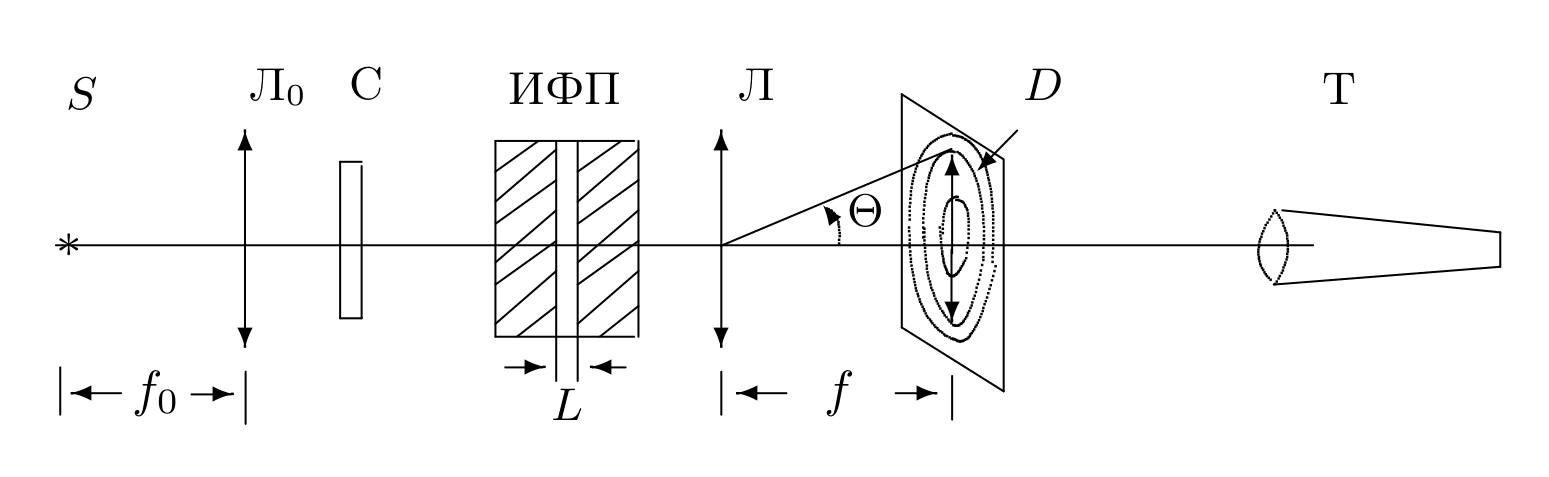
\includegraphics[width=\linewidth]{UST.png}}
  \caption{Схема экспериментальной установки}
  \label{img::3}
\end{figure}

При достаточной яркости ртутной лампы можно увидеть, что зелёная линия ртути состоит из 
нескольких компонентов. Расщепление этой спектральной линии связано с дополнительной энергией,
возникающей как в результате взаимодействия магнитных моментов ядра и электрона -- сверхтонкая
структура (магнитное поле ядра действует на спиновый магнитный момент электрона), так и с
изотопическим сдвигом (в парах ртути присутствуют в заметных количествах изотопы с атомными 
массами от 198 до 204 а.е.м.). Каждое зелёное кольцо содержит более десятка близко 
расположенных компонент, но разрешение нашего прибора не позволяет все их рассмотреть.
Спектр натриевой лампы исследуется по аналогичной схеме, но светофильтр в этом случае не нужен, 
а интерферометр, линзы и зрительная труба катетометра имеют другие параметры.